% Also note that the "draftcls" or "draftclsnofoot", not "draft", option
% should be used if it is desired that the figures are to be displayed in
% draft mode.
%

\setlength{\paperheight}{11in}
\setlength{\paperwidth}{8.5in}

%\documentclass[conference]{IEEEtran}
%\documentclass{acm_proc_article-sp}
\documentclass{sig-alternate}

% correct bad hyphenation here
\hyphenation{op-tical net-works semi-conduc-tor}

% Optionally save space in lists (place this command after a list environment (e.g., itemize, enumerate, description)
\newcommand{\compresslist}{
	\vspace{-.5em}
	\setlength{\itemsep}{1pt}
	\setlength{\parskip}{0pt}
	\setlength{\parsep}{0pt}
}

\usepackage{flushend}

\usepackage{listings}
\usepackage{subfigure}
\usepackage{cite}
\usepackage{url}
\usepackage{tabularx}
\usepackage[table, svgnames]{xcolor} 
\usepackage{color}
\usepackage{siunitx}
\usepackage{multirow}
\usepackage{wasysym}
\usepackage{times}
\usepackage{graphicx}
\usepackage{epsf}
\usepackage{verbatim}
\usepackage{psfig}
\usepackage{cite}
\usepackage{url}
\usepackage{color}
\usepackage[table]{xcolor}
\usepackage{booktabs, dcolumn}
\usepackage{alltt}

\usepackage{longtable,lscape}
\usepackage{slashbox,multirow}
\usepackage{colortbl}
\usepackage{mathrsfs}

\newcommand{\Add}{\CodeIn{add}}
\newcommand{\AVTree}{\CodeIn{AVTree}}
\newcommand{\Assignment}[3]{$\langle$ \Object{#1}, \Object{#2}, \Object{#3} $\rangle$}
\newcommand{\BinaryTreeRemove}{\CodeIn{BinaryTree\_remove}}
\newcommand{\BinaryTree}{\CodeIn{BinaryTree}}
\newcommand{\Caption}{\caption}
\newcommand{\Char}[1]{`#1'}
\newcommand{\CheckRep}{\CodeIn{checkRep}}
\newcommand{\ClassC}{\CodeIn{C}}
\newcommand{\CodeIn}[1]{{\small\texttt{#1}}}
\newcommand{\CodeOutSize}{\scriptsize}
\newcommand{\Comment}[1]{}
\newcommand{\Ensures}{\CodeIn{ensures}}
\newcommand{\ExtractMax}{\CodeIn{extractMax}}
\newcommand{\FAL}{field-ordering}
\newcommand{\FALs}{field-orderings}
\newcommand{\Fact}{observation}
\newcommand{\Get}{\CodeIn{get}}
\newcommand{\HashSet}{\CodeIn{HashSet}}
\newcommand{\HeapArray}{\CodeIn{HeapArray}}
\newcommand{\Intro}[1]{\emph{#1}}
\newcommand{\Invariant}{\CodeIn{invariant}}
\newcommand{\JUC}{\CodeIn{java.\-util.\-Collections}}
\newcommand{\JUS}{\CodeIn{java.\-util.\-Set}}
\newcommand{\JUTM}{\CodeIn{java.\-util.\-TreeMap}}
\newcommand{\JUTS}{\CodeIn{java.\-util.\-TreeSet}}
\newcommand{\JUV}{\CodeIn{java.\-util.\-Vector}}
\newcommand{\JMLPlusJUnit}{JML+JUnit}
\newcommand{\Korat}{Korat}
\newcommand{\Left}{\CodeIn{left}}
\newcommand{\Lookup}{\CodeIn{lookup}}
\newcommand{\MethM}{\CodeIn{m}}
\newcommand{\Node}[1]{\CodeIn{N}$_#1$}
\newcommand{\Null}{\CodeIn{null}}
\newcommand{\Object}[1]{\CodeIn{o}\ensuremath{_#1}}
\newcommand{\PostM}{\MethM$_{post}$}
\newcommand{\PreM}{\MethM$_{pre}$}
\newcommand{\Put}{\CodeIn{put}}
\newcommand{\Remove}{\CodeIn{remove}}
\newcommand{\RepOk}{\CodeIn{repOk}}
\newcommand{\Requires}{\CodeIn{requires}}
\newcommand{\Reverse}{\CodeIn{reverse}}
\newcommand{\Right}{\CodeIn{right}}
\newcommand{\Root}{\CodeIn{root}}
\newcommand{\Set}{\CodeIn{set}}
\newcommand{\State}[1]{2^{#1}}
\newcommand{\TestEra}{TestEra}
\newcommand{\TreeMap}{\CodeIn{TreeMap}}

\newenvironment{CodeOut}{\begin{scriptsize}}{\end{scriptsize}}
\newenvironment{SmallOut}{\begin{small}}{\end{small}}

\newcommand{\pairwiseEquals}{PairwiseEquals}
\newcommand{\monitorEquals}{MonitorEquals}
%\newcommand{\monitorWField}{WholeStateW}
\newcommand{\traverseField}{WholeState}
\newcommand{\monitorSMSeq}{ModifyingSeq}
\newcommand{\monitorSeq}{WholeSeq}

\newcommand{\IntStack}{\CodeIn{IntStack}}
\newcommand{\UBStack}{\CodeIn{UBStack}}
\newcommand{\BSet}{\CodeIn{BSet}}
\newcommand{\BBag}{\CodeIn{BBag}}
\newcommand{\ShoppingCart}{\CodeIn{ShoppingCart}}
\newcommand{\BankAccount}{\CodeIn{BankAccount}}
\newcommand{\BinarySearchTree}{\CodeIn{BinarySearchTree}}
\newcommand{\LinkedList}{\CodeIn{LinkedList}}

\newcommand{\Book}{\CodeIn{Book}}
\newcommand{\Library}{\CodeIn{Library}}

\newcommand{\Jtest}{Jtest}
\newcommand{\JCrasher}{JCrasher}
\newcommand{\Daikon}{Daikon}
\newcommand{\JUnit}{JUnit}

\newcommand{\trie}{trie}

\newcommand{\Perl}{Perl}


\newcommand{\SubjectCount}{11}
\newcommand{\DSSubjectCount}{two}

\newcommand{\Equals}{\CodeIn{equals}}
\newcommand{\Pairwise}{PairwiseEquals}
\newcommand{\Subgraph}{MonitorEquals}
\newcommand{\Concrete}{WholeState}
\newcommand{\ModSeq}{ModifyingSeq}
\newcommand{\Seq}{WholeSeq}
\newcommand{\Aeq}{equality}

\newcommand{\Meaning}[1]{\ensuremath{[\![}#1\ensuremath{]\!]}}
\newcommand{\Pair}[2]{\ensuremath{\langle #1, #2 \rangle}}
\newcommand{\Triple}[3]{\ensuremath{\langle #1, #2, #3 \rangle}}
\newcommand{\SetSuch}[2]{\ensuremath{\{ #1 | #2 \}}}

\newcommand{\Equiv}[2]{\ensuremath{#1 \EquivSTRel{} #2}}
\newcommand{\EquivME}{\Equiv}
\newcommand{\EquivST}{\Equiv}
\newcommand{\EquivSTRel}{\ensuremath{\cong}}
\newcommand{\Redundant}[2]{\ensuremath{#1 \lhd #2}}
\newcommand{\VB}{\ensuremath{\mid}}
\newcommand{\MES}{method-entry state}

\newcommand{\Small}[1]{{\small{#1}}}

\newcommand{\CenterCell}[1]{\multicolumn{1}{c|}{#1}}

% Yoonki's code
\colorlet{tableheadcolor}{gray!25} % Table header colour = 25% gray
\newcommand{\headcol}{\rowcolor{tableheadcolor}} %
\colorlet{tablerowcolor}{gray!10} % Table row separator colour = 10% gray
\newcommand{\rowcol}{\rowcolor{tablerowcolor}} %
    % Command \topline consists of a (slightly modified) \toprule followed by a \heavyrule rule of colour tableheadcolor (hence, 2 separate rules)
\newcommand{\topline}{\arrayrulecolor{black}\specialrule{0.1em}{\abovetopsep}{0pt}%
            \arrayrulecolor{tableheadcolor}\specialrule{\belowrulesep}{0pt}{0pt}%
            \arrayrulecolor{black}}
    % Command \midline consists of 3 rules (top colour tableheadcolor, middle colour black, bottom colour white)
\newcommand{\midline}{\arrayrulecolor{tableheadcolor}\specialrule{\aboverulesep}{0pt}{0pt}%
            \arrayrulecolor{black}\specialrule{\lightrulewidth}{0pt}{0pt}%
            \arrayrulecolor{white}\specialrule{\belowrulesep}{0pt}{0pt}%
            \arrayrulecolor{black}}
    % Command \rowmidlinecw consists of 3 rules (top colour tablerowcolor, middle colour black, bottom colour white)
\newcommand{\rowmidlinecw}{\arrayrulecolor{tablerowcolor}\specialrule{\aboverulesep}{0pt}{0pt}%
            \arrayrulecolor{black}\specialrule{\lightrulewidth}{0pt}{0pt}%
            \arrayrulecolor{white}\specialrule{\belowrulesep}{0pt}{0pt}%
            \arrayrulecolor{black}}
    % Command \rowmidlinewc consists of 3 rules (top colour white, middle colour black, bottom colour tablerowcolor)
\newcommand{\rowmidlinewc}{\arrayrulecolor{white}\specialrule{\aboverulesep}{0pt}{0pt}%
            \arrayrulecolor{black}\specialrule{\lightrulewidth}{0pt}{0pt}%
            \arrayrulecolor{tablerowcolor}\specialrule{\belowrulesep}{0pt}{0pt}%
            \arrayrulecolor{black}}
    % Command \rowmidlinew consists of 1 white rule
\newcommand{\rowmidlinew}{\arrayrulecolor{white}\specialrule{\aboverulesep}{0pt}{0pt}%
            \arrayrulecolor{black}}
    % Command \rowmidlinec consists of 1 tablerowcolor rule
\newcommand{\rowmidlinec}{\arrayrulecolor{tablerowcolor}\specialrule{\aboverulesep}{0pt}{0pt}%
            \arrayrulecolor{black}}
    % Command \bottomline consists of 2 rules (top colour
\newcommand{\bottomline}{\arrayrulecolor{white}\specialrule{\aboverulesep}{0pt}{0pt}%
            \arrayrulecolor{black}\specialrule{\heavyrulewidth}{0pt}{\belowbottomsep}}%
\newcommand{\bottomlinec}{\arrayrulecolor{tablerowcolor}\specialrule{\aboverulesep}{0pt}{0pt}%
            \arrayrulecolor{black}\specialrule{\heavyrulewidth}{0pt}{\belowbottomsep}}%

\usepackage{dcolumn}
\newcolumntype{Y}{D..{6.4}}

%\newcommand{\blind}[1]{{\color{white}\{#1\}}}
\newcommand{\blind}[1]{#1}

\clubpenalty = 10000
\widowpenalty = 10000
\displaywidowpenalty = 10000

%
% paper title
% can use linebreaks \\ within to get better formatting as desired
% Do not put math or special symbols in the title.
\begin{document}
\toappear{}
%Strategic analysis of static analysis defect resolution
%Analyzing, supporting?
%Straticheck: Identifying Successful Strategies for Resolving IDE Notifications
%Helping developers uses\ successful strategies to resolve static analysis notifications
\title{Identifying Successful Strategies for Resolving Static Analysis Notifications}

\numberofauthors{1}
\author{
\alignauthor Justin Smith\\
\affaddr{North Carolina State University}\\
\affaddr{Raleigh, NC, USA} \\
\email{jssmit11@ncsu.edu}
}

\maketitle


\begin{abstract}
Static analysis tools have increasingly drawn attention from the research community because they afford the early detection of potential code defects.
However, resolving these defects often requires considerable effort from developers.
Unfortunately, research findings suggest static analysis tools don't fully support developers in resolving the defects the tools detect.
In this work I examine the ad-hoc strategies developers use to resolve defects. 
Further, I present a tool that explicates strategies.
[Obviously more work to do here]

\end{abstract}

% % A category with the (minimum) three required fields
% \category{H.4}{Information Systems Applications}{Miscellaneous}
% %A category including the fourth, optional field follows...
%\category{D.2.6}{Software Engineering}{Programming Environments}
%\keywords{XXXXX}

\section{Introduction}
\label{sec:intro}
Static analysis tools help developers locate various code defects early in the development process, even before the code executes. 
For example, static analysis tools detect access control vulnerabilities~\cite{Aside}, potential null dereferences~\cite{FindBugs}, and concurrency bugs~\cite{ThreadSafe} by analyzing source code.
Detecting, and more importantly, resolving defects like these early can prevent more costly failures later in the development process~\cite{ayewah2008using}.

In their defect reports, static analysis tools provide information to developers in the form of textual \textit{notifications}.
These notifications typically describe possible defects.
However, they often fail to fully support developers in actually resolving the defects they detect~\cite{Johnson2013}.
For example, accurately resolving defects can require developers to identify false positives, explore the existing code, invoke additional tools, modify the code, and verify the correctness of their fix, among other additional activities~\cite{Smith2015}.  
Even with notifications that afford actionable ``Quick Fix'' suggestions, developers must still determine whether those suggestions are appropriate for their code.
Consider one of the most common \cite{Ayewah2007} notifications produced by FindBugs, a static analysis tool, which in this case, does not provide any imperative suggestions:

%\begin{lstlisting}[language=Java, keywordstyle=\color{blue}]
%object.add("foo");
%if (object != null){
% object.add("foo");
%}
%\end{lstlisting}

\vspace{2mm}

\begin{tabular}{|p{7.5cm}}
	``There is a branch of statement that, if executed, guarantees that a null value will be dereferenced, which would generate a NullPointerException when the code is executed. Of course, the problem might be that the branch or statement is infeasible and that the null pointer exception can't ever be executed; \textbf{deciding that is beyond the ability of FindBugs.}"\\
\end{tabular}
\vspace{2mm}

\noindent
The notification clearly identifies the problem with the code (a null value may be dereferenced), however the notification provides no suggestions about how the developer should proceed to resolve the defect. 

The actions developers take to resolve defects, I refer to collectively as the developer's defect resolution \textit{strategy}.
For example, one strategy for resolving this defect would be to use Google to search for information about NullPointerExceptions, use Eclipse's call hierarchy tool to explore which branches get executed, and finally add an additional null check only if deemed appropriate.
Of course, there exist other strategies for resolving this defect.

I envision an alternative paradigm in which static analysis tool notifications explicitly support the resolution of the defects they detect. 
In particular, I envision a tool that supports successful defect resolution strategies by orchestrating the actions developers take and tools developers use to resolve defects.
In this paper, I contribute: 
\begin{enumerate}
	\compresslist
	\item A preliminary analysis of the successful and unsuccessful strategies developers employ to resolve defects detected by static analysis, and
	\item A description of a tool that provides developers with the tools and strategies needed to resolve defects.
	
\end{enumerate}

%When interacting with a given static analysis notification, a developer's current task is well known. I can leverage that knowledge to provide context sensitive information about effective strategies.

\section{Related Work}
\label{sec:rw}
%In this section, I briefly survey related work.
%\subsection{Defect Resolution}
Several researchers have stressed the importance of static analysis tools supporting defect resolution, not just detection.
For example, Path Projection~\cite{Khoo2008} facilitates defect resolution by presenting program path visualizations. 
Similarly, Quick Fix Scout~\cite{Muslu2012} supports defect resolution by performing speculative analysis and therefore enabling developers to preview and compare fixes.
Taken alone, Path Projection and Quick Fix Scout each only support one step in the defect resolution process.
In this work, I envision an approach that supports developers throughout every step of the defect resolution process by orchestrating tools that focus on supporting individual steps.

%\subsection{Supporting Effective Strategies}
Previous research has also focused on the importance of supporting successful strategies in the use of complex computer applications.
In computer-aided design applications, for example, Bhavnani and John have measured the performance costs of inefficient strategies~\cite{Bhavnani2000}.
Their results suggest the use of more efficient strategies leads to faster task completion time and more accurate results.
They also show that offline educational interventions can increase the use of efficient strategies.
Leaning on the work of Bhavnani and John, Cockburn and colleagues review interface research and state that knowledge of efficient strategies is also an important factor influencing the novice to expert transition~\cite{Cockburn2014}.
In his work, Cockburn discusses several techniques for designing interfaces that implicitly encourage the use of efficient strategies.
These research efforts emphasize the importance of educating users about efficient strategies, however neither proposes to do so by explicitly prescribing effective strategies to users while they complete the relevant task.
Building off this previous work, my approach aims to proliferate strategic knowledge by explicitly describing successful strategies. 

%rather than designing systems that implicitly encourage them.

%In resloving defects this is feasible, because the specific task is know a priori


%In other disciplines, the explanation of successful strategies is critical to the accurate completion of tasks. In the natural sciences, lab protocols are written guidelines that describe strategies for successfully completing an experiment. Recently, Abbott and colleagues examined the parallels between lab protocols and mixed initiative systems [Cite VL/HCC paper]. 

%For example, in the culinary arts recipes capture all of the strategic information needed to complete cooking tasks~\cite{Recipes2013}.



 %Brittany's stuff, my stuff
 
 
 %Unlike complex applications that Bhavnani and John studied, 



\section{Approach}
\label{sec:approach}
To enable tools to explicitly support developers in executing efficient defect resolution strategies, I must first identify the successful strategies those tools should support. 


%\subsection{Analyze existing notifications for strategy support?}
%Debating adding another section here, but will want to discuss in reading group.
%Analyze all FB messages to determine to what extent static analysis notifications support holistic fixes
%how actionable?
%Only X\% of FindBugs notifications include information about how to resolve the defect. 

%

\subsection{Identifying Successful Strategies}
In previous work, I conducted a study in which ten developers each worked towards resolving four defects using static analysis~\cite{Smith2015}.
In particular, developers in the study interacted with security defects detected by Find Security Bugs~\cite{FindSecurityBugs} --- a security-oriented extension of FindBugs~\cite{FindBugs}.
As part of this previous work, I identified the information developers needed while resolving these defects.

In the absence of tool-sanctioned defect resolution strategies, developers executed ad-hoc strategies (with varying degrees of success) to gather the information they needed.
In this work I focus on identifying those successful and unsuccessful ad-hoc strategies.
%Goms task decomposition??
To that end, I reanalyzed the audio and video recordings from ~\cite{Smith2015}. 

Returning to the example of a defect resolution strategy from Section~\ref{sec:intro}, which is notably more concise than the strategies I observed in this study, Figure~\ref{fig:description} depicts the notation I would use to describe the defect resolution strategy. 
Similar to the notion of attack trees~\cite{attackTrees}, which hierarchically depict the actions an attacker could take to exploit a system, this hierarchical representation describes defect resolution strategies as a structured sets of actions.
Because different developers might used different strategies to resolve the same defect, I constructed one of these strategy trees for each individual task I observed in the study --- 40 in total.
Finally, to measure success granularly, I annotated a strategy in the tree whenever it either contributed to or detracted from the accurate resolution of the defect (lines prefixed with +/-, respectively, in Figure \ref{fig:description}).


\begin{figure}
	\centering
	\includegraphics[width=\columnwidth]{"strategy description format"}
	\caption{Abbreviated description of a strategy for resolving a null dereference defect, including example annotations of observed points of success/failure (marked with +/- in green and red, respectively). }
	\label{fig:description} 

\end{figure}


%\subsection{Supplementing Observed Strategies}

%Since the developers I observed range in experience levels and may not have executed all of the most successful strategies, I supplement the observed strategies by examining defect resolution strategies published by trusted authorities. In particular, I incorporated information published by OWASP and the CVE.

%



\section{Results}
I identified 40 strategies for defect resolution across 4 types of security defects. 
Not surprisingly, the strategies I observed vary depending on the individual developer.
For example, the three developers who reported the least familiarity with security vulnerabilities started 11 of the 12 tasks by reading the notification text.
In contrast, more experienced developers started by reading the code.
The two developers who reported the highest familiarity with security vulnerabilities started only 2 of 8 tasks by reading the notification text. 
%Inexperience read the notification. Promising for our intervention

Though all the strategies I identified exhibit slight differences (such as how developers chose to start resolving the defect), some common patterns emerged across participants and defects. 
In all 40 strategies, developers read the code surrounding the defect. Furthermore, in 90\% of the strategies developers read the notification text and in 75\% of the strategies developers tried to determine if the notification was a false positive.
The existence of these patterns is promising, because it may point to the feasibility of recommending strategies that apply more broadly. 
%At least given a defect?
%Some underlying patterns possible to suggest strategies that apply generally
%Promising, because it may suggest the possibility of sharing strategies across developers.

Examining the strategies based on the degree to which they lead to successful outcomes, I observed 55 [TODO:Update This Number] strategic failures (i.e, instances where a developer's strategy was not efficient or accurate). Some examples of strategic failures include: the developer making an incorrect inference, using a tool incorrectly, or proposing an incorrect code modification.
I observed at least one strategic failure in 22 of 30[TODO:Update this] tasks; across the four tasks, every developer's strategies were undermined by at least one failure.
However, despite the lack of tool support, some developers did resolve defects correctly using successful strategies. I observed 90 instances where developers' defect resolution strategies were successful in leading them to make observable progress on the resolution task.

Drawing from the successful strategies I observed, I sketched (Figure~\ref{fig:tool}) a tool that presents explicit defect resolution strategies to the developer. 
The strategy this tool presents is a composite strategy, combining the ten strategies I observed developers using for one task.
Since the developers I studied may not have executed all of the most successful strategies, I supplement the tool by also including defect resolution recommendations published by trusted authorities such as OWASP and CVE~\cite{OWASP, CVE}.
The tool also includes checkboxes to allow developers to track their progress.
Additionally, (talk about invoking other tools)

\section{Contributions}
%Use in practice to ensure tasks are completed successfully, or in education to disseminate strategic knowledge


In this section I restate my contributions from the intro...

%work I present a tool, Strategy-Check, that embraces this paradigm by explicating successful strategies in the form of hierarchically structured checklists;


\begin{figure}
	\centering
	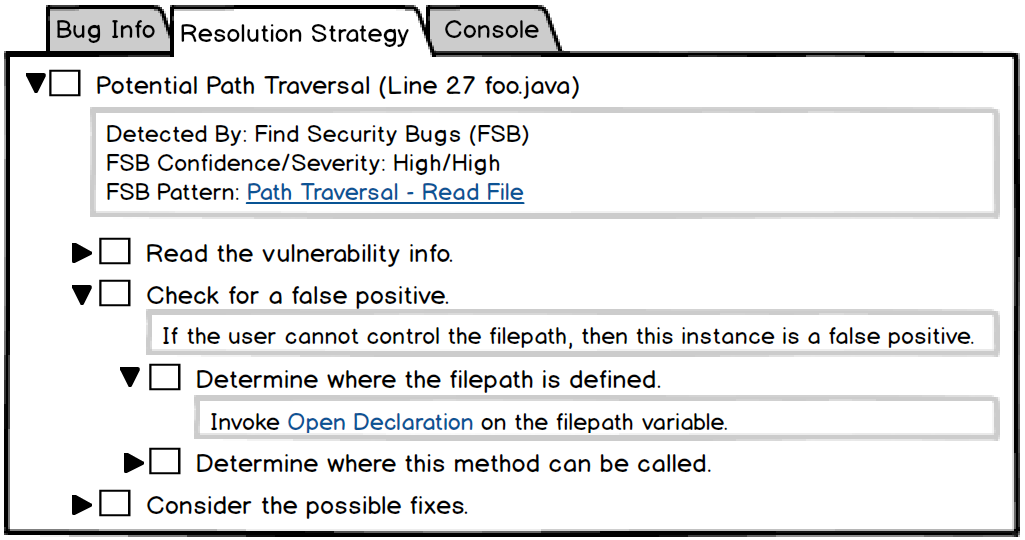
\includegraphics[width=\columnwidth]{images/toolscreenshot}
	\caption{A mockup of a tool that presents successful strategies.}
	\label{fig:tool} 
\end{figure}



\bibliographystyle{abbrv}
\bibliography{Strategy-Encapsulation-Paper}
%
% <OR> manually copy in the resultant .bbl file
% set second argument of \begin to the number of references
% (used to reserve space for the reference number labels box)


% that's all folks
\end{document}


